%!TEX root = mainfile.tex

\section{Introduction} % (fold)
\label{sec:introduction}
	Tomography is a technique for imaging objects and examining the internal structure of them in a non-invasive way. It is of enormous use in the medical industry where the ability to view the inside of a patient's body can be invaluable in the diagnostic process. Tomography stands out from other methods of viewing the internal structures of objects since it is able to view a slice through the object without the addition of the material around it in other slices, i.e.\ the rest of the object does not obscure the slice being viewed.

    Tomography can be applied to many different imaging techniques, x-ray, MRI and ultrasound, and has been applied to many areas of scientific study and research including medicine, chemistry, astronomy and geology.

    Tomographic reconstruction involves the creation of an image of an object taken through a particular slice by recombining the data collected from a set of line integrals across that object in the plane of interest. In other words, it is the conversion of a 3D averaged, or integrated, view of an object into a 2D slice of the object at a particular location, so that the details of the interior can be examined.

    The word tomography comes from the Greek \textit{tomos} meaning section and \textit{graphein} meaning to write, so tomography is simply writing `parts' of an object, in this case an image of a single plane through that object, in a useful form.
% section introduction (end)

\section{Tomographic Reconstruction} % (fold)
\label{sec:tomographic_reconstruction}
    In order to examine this method of image construction, we shall use a series of images which form \textit{sagittal} slices of a human head. This means that each of the 129 images in the collection are a slice from side to side at a slightly different position. Together, they form a 3 dimensional image of the head, with all of the interior detail maintained. A few of these images are shown in figure~\ref{fig:example_sagittal}
    \begin{figure}[ht]
        \centering
        \begin{minipage}[c]{0.19\linewidth}
            \centering
            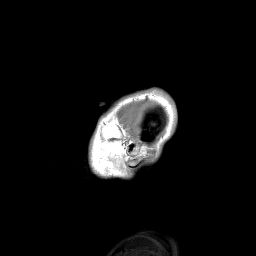
\includegraphics[width=\textwidth]{Files/report_images/sagittal_example1.jpg}
        \end{minipage}
        \begin{minipage}[c]{0.19\linewidth}
            \centering
            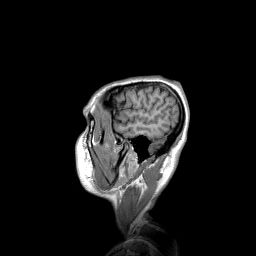
\includegraphics[width=\textwidth]{Files/report_images/sagittal_example2.jpg}
        \end{minipage}
        \begin{minipage}[c]{0.19\linewidth}
            \centering
            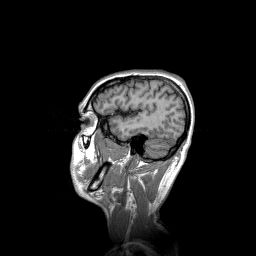
\includegraphics[width=\textwidth]{Files/report_images/sagittal_example3.jpg}
        \end{minipage}
        \begin{minipage}[c]{0.19\linewidth}
            \centering
            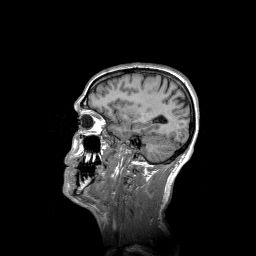
\includegraphics[width=\textwidth]{Files/report_images/sagittal_example4.jpg}
        \end{minipage}
        \begin{minipage}[c]{0.19\linewidth}
            \centering
            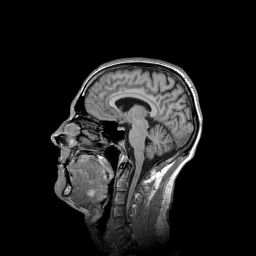
\includegraphics[width=\textwidth]{Files/report_images/sagittal_example5.jpg}
        \end{minipage}
        \caption{Example slices from the original sagittal 3D image that will be used to examine the tomographic reconstruction method. Out of the 129 images that make up the full image, these are, from left to right, image 20, 31. 38, 48 and 64 respectively.\label{fig:example_sagittal}}
    \end{figure}

    In order to demonstrate the tomographic reconstruction method as used in medical applications, an effective CT scan can be taken of this 3D image by converting it to axial slices. These are slices taken laterally through the object from top to bottom. Again, a selection of this new 3D image is shown in figure~\ref{fig:example_axial}.
    \begin{figure}[ht]
        \centering
        \begin{minipage}[c]{0.3\linewidth}
            \centering
            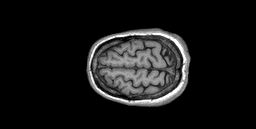
\includegraphics[width=\textwidth]{Files/report_images/axial_example1.jpg}
        \end{minipage}
        \begin{minipage}[c]{0.3\linewidth}
            \centering
            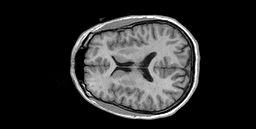
\includegraphics[width=\textwidth]{Files/report_images/axial_example2.jpg}
        \end{minipage}
        \begin{minipage}[c]{0.3\linewidth}
            \centering
            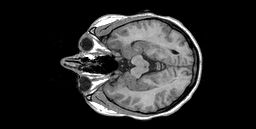
\includegraphics[width=\textwidth]{Files/report_images/axial_example3.jpg}
        \end{minipage}

        \begin{minipage}[c]{0.3\linewidth}
            \centering
            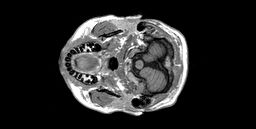
\includegraphics[width=\textwidth]{Files/report_images/axial_example4.jpg}
        \end{minipage}
        \begin{minipage}[c]{0.3\linewidth}
            \centering
            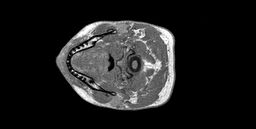
\includegraphics[width=\textwidth]{Files/report_images/axial_example5.jpg}
        \end{minipage}
        \begin{minipage}[c]{0.3\linewidth}
            \centering
            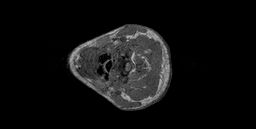
\includegraphics[width=\textwidth]{Files/report_images/axial_example6.jpg}
        \end{minipage}
        \caption{Example slices from the original sagittal 3D image that will be used to examine the tomographic reconstruction method. Out of the 129 images that make up the full image, these are, from top left to bottom right, image 78, 106, 126, 162 and 182 respectively.\label{fig:example_axial}}
    \end{figure}

    In order to show the effectiveness of the different techniques used in tomographic reconstruction, we shall refer back to a single of these slices, which will be the one that shall be reconstructed. This reference image will be image NUM out of the 256 stack above, and is shown in figure~\ref{fig:reference_slice}.
    \begin{figure}[ht]
        \centering
        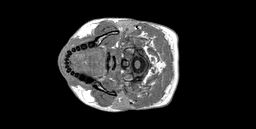
\includegraphics[width=0.4\textwidth]{Files/report_images/reference_slice.jpg}
        \caption{Reference slice that shall be used to compare later.\label{fig:reference_slice}}
    \end{figure}

    \subsection{Tomographic Scanner} % (fold)
    \label{sub:tomographic_scanner}
        When used in medical imaging applications, the data that is collected by a tomographic scanner would be represented by the image in figure~\ref{fig:3d_scan_example}.
        \begin{figure}[ht]
            \centering
                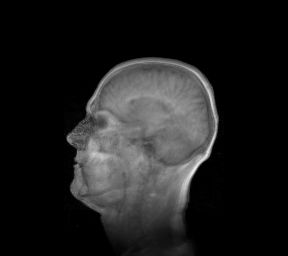
\includegraphics[width=0.4\textwidth]{Files/report_images/3D_scan_example.jpg}
            \caption{An image of the 3 dimensional representation of an object that would be measured by a tomographic scanner. This is just one view of the $360^{\circ}$ image that is generated.\label{fig:3d_scan_example}}
        \end{figure}

        The full image consists of a number of views of the object, each showing what it looks like from a different angle, averaged or integrated over its depth. Tomographic reconstruction involves calculating the reference image above, starting from this 3D representation
    % subsection tomographic_scanner (end)
% section tomographic_reconstruction (end)

\section{Back Projection} % (fold)
\label{sec:back_projection}
    The general method for tomographic reconstruction is called back projection. There are number of variations on this method that provide varying quality of results. We shall first examine the basic method of back projection and then see how it can be improved to increase the accuracy of the images calculated with it.

    \subsection{Sinogram} % (fold)
    \label{sub:sinogram}
        Since we now have a 3D image, such as would be collected when imaging an object from a large number of different angles around it, we can no longer determine what the interior contains. The first step to finding this is the plot a sinogram. Each slide of the 3D image is a view of the object from a particular angle. Since we require to see the interior of the object only through a particular single slice, most of the 3D image is not needed. Thus the useful information is a series of single pixel tall images of a single slice of the object taken at slightly different angle around it.

        A sinogram is a combined image of all of these views plotted as the value of the line integral with $x'$ against the angle $theta$, as per the diagram in figure~\ref{fig:sinogram_diag}. Since the different views are all taken about a single static point, polar co-ordinates are used, such that
        \begin{align}
            x\cos(\theta) + y\sin(\theta) = x'
        \end{align}
        Thus, the set of measurements that are collected for a given angle, $\theta$, make up a single layer of figure~\ref{fig:example_sinogram} and are called the parallel projection of the object at the angle $\theta$, denoted as $P_{\theta}(x')$.
        \begin{figure}[ht]
            \begin{center}
                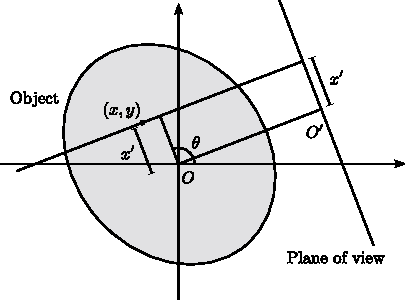
\includegraphics[width=0.5\textwidth]{Files/report_images/sinogram_diag.pdf}
            \end{center}
            \caption{A sinogram is an image of the value of the line integral plotted against angle for all the views around a measured object. Each point from the object traces a sinusoidal line as the angle is increased, or as the object is rotated in front of the measuring device. Angle is represented on the vertical axis and the position $x'$ on the horizontal.\label{fig:sinogram_diag}}
        \end{figure}

        An example of a sinogram, showing the plot for the data concerning the slice that holds the information for the reference image above, is shown in figure~\ref{fig:example_sinogram}.
        \begin{figure}[ht]
            \begin{center}
                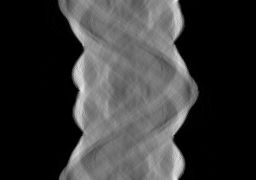
\includegraphics[width=0.4\textwidth]{Files/report_images/example_sinograph.jpg}
            \end{center}
            \caption{A sinogram is an image of the value of the line integral plotted against angle for all the views around a measured object. Each point from the object traces a sinusoidal line as the angle is increased, or as the object is rotated in front of the measuring device.\label{fig:example_sinogram}}
        \end{figure}

        \subsubsection{Radon Transform} % (fold)
        \label{ssub:radon_transform}
            The mathematical operation that gives the sinogram of an imaged slice is called the Radon Transform, ``it is the integral transform consisting of the integral of a function over straight lines''. In other words, the Radon Transform is the line integral along each of the possible straight lines defined over the area of the space represented by the original function. The transform is defined over the line space, $L$, as
            \begin{align}
                R_f(L) &= \int_L f(\boldsymbol{r})|\d{\boldsymbol{r}}|
            \end{align}
            Any stright line through the original function space can be defined in polar co-ordinates given a point through which the line passes and an angle $\theta$, that the line subtends. If the line passes through the point $(x,y)$, then any line can be defined as
            \begin{align}
                (x,y) &= \Big(\big[x'\cos(\theta)+y'\sin(\theta)\big], \big[-y'\cos(\theta)+x'\sin(\theta)\big]\Big)
            \end{align}
            where $x'$ is the distance of the line from the origin, as shown in figure~\ref{fig:sinogram_diag}. This means, then, that the Radon transform can be rewritted in terms of this general line form,
            \begin{align}
                R_f(\theta,x') &= \int_{-\infty}^{\infty} f(x,y)\d{t} \\
                &= \int_{-\infty}^{\infty} f\Big(\big[x'\cos(\theta)+y'\sin(\theta)\big], \big[-y'\cos(\theta)+x'\sin(\theta)\big]\Big)\d{t}
            \end{align}
            This means that every point in the original function is mapped to a location described by a combination of sine and cosine functions. This is clearly seen when considering the Radon Transform of several a Dirac Delta functions $\delta(x,y)$, which are described by the same number of sine waves with different phases, depending on their original position, as shown in figure~\ref{fig:delta_radon_transform}.
            \begin{figure}[ht]
                \centering
                \begin{minipage}[c]{0.2\linewidth}
                    \centering
                    
\includegraphics[width=\textwidth]{Files/report_images/radon_transform_deltas_original.png}
                \end{minipage}
                ~
                \begin{minipage}[c]{0.5\linewidth}
                    \centering
                    
\includegraphics[width=\textwidth]{Files/report_images/radon_transform_deltas.png}
                \end{minipage}
                \caption{The Radon Transform (left) of a series of finite delta functions (right). The Radon Transform can be thought of as the project of the original image as viewed from in the plane of the image, as the field of view is rotated around the image. The horizontal axis is now representing angle and vertical position.\label{fig:delta_radon_transform}}
            \end{figure}

            When this transform is applied to more complex images, the result is a very large number of blurred sine waves with different phases and also different amplitudes that, together, represent the whole image.
        % subsubsection radon_transform (end)
        \subsection{Back Projection Algorithm} % (fold)
        \label{sub:back_projection_algorithm}
            The basic steps when reconstructing the axial slice from the sinogram using back projection are as follows
            \begin{enumerate}
                \item Take the measured line integral at each offset along the projection
                \item Spread this value back uniformly along the line of measurement
                \item Repeat for every projection taken at all angles around the object
                \item Sum the contributions from all of the projections to give a back-projected reconstruction of the axial slice.
            \end{enumerate}

            This process is simple and computationally simple. However, this method produces serious artefacts making the image only just recognisable as the desired reconstruction, when compared to the reference image above, as shown in figure~\ref{fig:simple_backprojection}.
            \begin{figure}[ht]
                \begin{center}
                    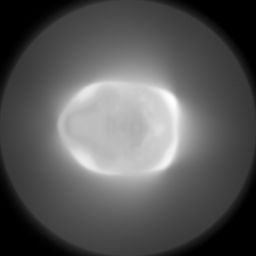
\includegraphics[width=0.4\textwidth]{Files/report_images/simple_backprojection.jpg}
                \end{center}
                \caption{The reconstructed axial slice using only basic back projection. The image is just recognisable as being related to the reference image, but there are severe artefacts and tails making any application of this image almost useless.\label{fig:simple_backprojection}}
            \end{figure}

            The reason the image looks so blurred, with so much extra information, is that the back-projections of each individual linear projection are summed over the full width and heigh of the image. This means that, although most, if not all, of the original information is concentrated in the centre of the image, this is spread out to include the edges, simply because there is nothing to tell the algorithm not to, and so the tails are spread back to the extremities of the image.

            We shall consider some methods for improving this image.
        % subsection back_projection_algorithm (end)
    % subsection sinogram (end)
% section back_projection (end)

\section{Central Slice Theorem} % (fold)
\label{sec:central_slice_theorem}
    The back projection method works, insofar as we now have an image, reconstructed from the 3D scan that is recognisable as the reference image in figure~\ref{fig:reference_slice}. However we want to improve the algorithm, so that it does not trace the projections back uniformly which leads to the long tails shown above. One method of doing this involves the central slice theorem.

    The Central Slice Theorem states that the results of the following two calculations are equal:
    \begin{itemize}
        \item Take a two-dimensional function $f(\boldsymbol{r})$, project it onto a one-dimensional line, and do a Fourier transform of that projection.
        \item Take that same function, but do a two-dimensional Fourier transform first, and then take a single slice through the origin, which is parallel to the projection line.
    \end{itemize}

    This theorem means that we can use each row of the sinogram to build the 2D Fourier Transform of the axial slice since the 1D Fourier Transform of each row forms a radial (central) slice of the 2D transform.
    \begin{figure}[ht]
        \begin{center}
            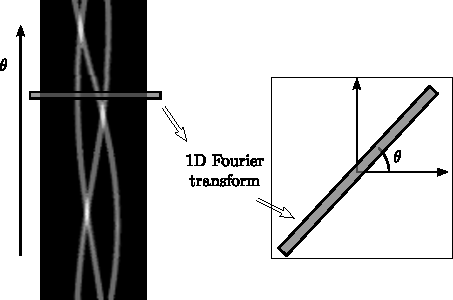
\includegraphics[width=0.6\textwidth]{Files/report_images/central_slice_theorem.pdf}
        \end{center}
        \caption{The central slice theorem means that the 2D Fourier Transform of the final image can be constructed from the 1D transforms of each slice of the sinogram.\label{fig:central_slice_theorem}}
    \end{figure}

    However, if this method is used to compute the axial slice, the same image as previously is found, with the tails and severe artefacts. This is because taking the Fourier Transform is a linear operation. This means that the steps taken here, taking the Fourier Transform (FT), adding the images and then taking the inverse FT is identical as adding the images and then taking the FT then the inverse FT. Since taking the FT and then inverse FT will clearly give the same original image, this is the same as before when just adding the back projections.

    The reason that there was no improvement in  final image quality is due to the distribution of samples of the Fourier Transform. Moving radially outward from the centre of the image, the sample density decreases as $\frac{1}{|r|}$, where $r$ is the radius. To correct for this, a weighting factor must be used to make the FT uniform in sample density. This is performed either in frequency space once the FT has been taken, before the inverse, or in real space.

    The weighting factor is usually applied in real space as this proves to be less computationally intensive. This is possible because multiplying each central slice by the weighting factor is the same as convolving the inverse FT of each slice with the inverse FT of the weighting factor. 

    We can demonstrate this by considering the Fourier Transform for both cases. The general function, $f(x,y)$ can be obtained from its Fourier Transform $F(k_x,k_y)$ by the inverse transform,
    \begin{align}
        f(x,y) &= \int_{-\infty}^{\infty}\int_{-\infty}^{\infty}F(k_x,k_y)\e{ik_xx+ik_yy} \d{k_x}\d{k_y}
    \end{align}
    Since the central slice theorem is defined through the centre of the transform, it is convenient to use polar coordinates, though with ranges $-\infty < k < \infty$ and $0 < \theta < \pi$,
    \begin{align}
        f(x,y) &= \int_{0}^{\pi}\int_{-\infty}^{\infty}F(k,\theta)|k|\e{ik(x\cos\theta + y\sin\theta)} \d{k}\d{\theta}
    \end{align}
    If we define $F(k,\theta) = Q_{\theta}(k)$, where $Q_{\theta}$ is the Fourier Transform of the projection $P_{\theta}$, then we have,
    \begin{align}
        f(x,y) &= \int_{0}^{\pi}\left\{\int_{-\infty}^{\infty}Q_{\theta}(k)|k|\e{ik(x\cos\theta + y\sin\theta)} \d{k}\right\}\d{\theta} \\
        &= \int_{0}^{\pi}\underbrace{\int_{-\infty}^{\infty}Q_{\theta}(k)|k|\e{ikx'} \d{k}}_\text{A}\d{\theta} \label{eq:filtered_backprojection}
    \end{align}
    This means that the image $f(x,y)$ can be found by back projecting part A of equation~\ref{eq:filtered_backprojection}. Part A is the inverse Fourier Transform of the two functions $Q_{\theta}$ and $|k|$, and so, since $Q_{\theta}$ is the the FT of $P_{\theta}$, A can be expressed as the convolution of $P_{\theta}$ with a filter given by the inverse FT of the weighting function. All that remains, then, in order to perform the reconstruction is to find the filter, given by the inverse FT of the weighting function. The 2D Fourier Transform of $\frac{1}{r}$ is $\frac{1}{|k|}$, and so the weighting function that is used as the filter is the inverse FT of $|k|$.

    \subsection{Filter} % (fold)
    \label{sub:filter}
        The function that we need to use as the filter, in order to correct for the changes in density of the FT sampling is the inverse FT of the function $|k|$. When considering the whole plane, from $-\infty < k < \infty$, this solution does not exist as the series diverges. But there is a maximum frequecy, $k$, that is of interest, the Nyquist Frequency outside of which the information can be disgarded, and so the function can be redefined as
        \begin{align}
            f(k) =
                \begin{cases}
                    |k| & |k| < k{_\text{max}} \\
                    0   & |k| > {_\text{max}}
                \end{cases}
        \end{align}
        The inverse FT for this function is defined as 
        \begin{align}
            f(x) &= k^2_{\text{max}} \left[ \frac{2\sin(2\pi xk_{\text{max}})}{2\pi xk_{\text{max}}} - \left( \frac{\sin(\pi xk_{\text{max}})}{\pi xk_{\text{max}}} \right)^2 \right]
        \end{align}
        and is shown in figure~\ref{fig:filter_graph}.
        \begin{figure}[ht]
            \centering
                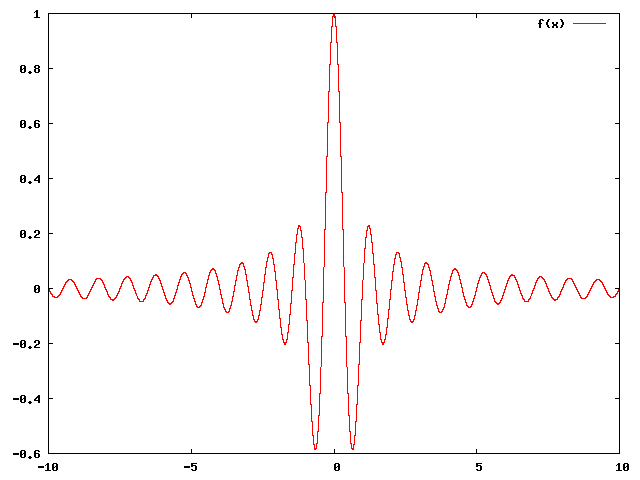
\includegraphics[width=0.7\textwidth]{Files/report_images/inverse_FT_filter.png}
            \caption{The filter used to weight the projections to remove the long tails that obscure the image.\label{fig:filter_graph}}
        \end{figure}
    % subsection filter (end)
    \subsection{Applying the Filter} % (fold)
    \label{sub:applying_the_filter}
        Applying the filter is performed by convolving it with the projections. Since the function is continuous, but the convolution kernel must be discrete, integer values are used, as shown by the dots in the graph in figure~\ref{fig:filter_graph}. The filter kernel is found by using the value of the filter function at these integer values of $x$ and is normalised so that the elements sum to zero.

        Using this method of convolving the inverse FT of the weighting function with the projections, projecting them back and then summing the result to reconstruct the original image produces the image in figure~\ref{fig:filtered_backprojection}.
        \begin{figure}[ht]
            \centering
                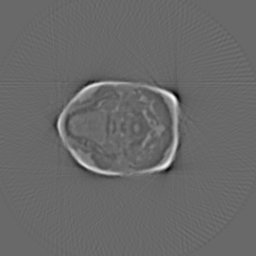
\includegraphics[width=0.4\textwidth]{Files/report_images/reconstructed_image.jpg}
            \caption{The filter used to weight the projections to remove the long tails that obscure the image.\label{fig:filtered_backprojection}}
        \end{figure}
    % subsection applying_the_filter (end)


% section central_slice_theorem (end)

